% This must be in the first 5 lines to tell arXiv to use pdfLaTeX, which is strongly recommended.
\pdfoutput=1
% In particular, the hyperref package requires pdfLaTeX in order to break URLs across lines.

\documentclass[11pt]{article}

\usepackage[a4paper, total={6in, 8in}, margin=0.7in]{geometry}
\usepackage{lineno}
\linenumbers

\usepackage{caption,subcaption}

\usepackage{mystyle}

\usetikzlibrary{calc,patterns,angles,quotes}    
\usetikzlibrary{decorations.pathmorphing}
\tikzset{snake it/.style={decorate, decoration=snake}}

\usepackage{natbib}
\bibliographystyle{abbrvnat}
\usepackage{hyperref}

% Standard package includes
\usepackage{times}
\usepackage{latexsym}

% For proper rendering and hyphenation of words containing Latin characters (including in bib files)
\usepackage[T1]{fontenc}
% For Vietnamese characters
% \usepackage[T5]{fontenc}
% See https://www.latex-project.org/help/documentation/encguide.pdf for other character sets

% This assumes your files are encoded as UTF8
\usepackage[utf8]{inputenc}


\title{Approximate Dynamic Programming for State Space Models}

\author{Justin Chiu \\
  Cornell Tech \\
  \texttt{jtc257@cornell.edu}}

\begin{document}
\maketitle
\begin{abstract}
A note where we apply value function estimation to gradient estimation in
state space models.
\end{abstract}

\section{Problem Setup}
The goal is to maximize expected rewards $\argmax_\pi \Es{a_{1:t},s_{1:t}\sim\pi}{\sum_{t=1}^T r(a_t, s_t)}$,
where actions $a_t\in A$ come from our policy $\pi$,
and states $s_t\in S$ may or may not be observable.
If states are observed, then this process is known as a Markov decision process (MDP).
If the state are not observable,
then we assume a simple observation model $o_t\in O \sim p(o_t \mid s_t, a_{t-1})$
(may be conditionally independent of actions $p(o_t \mid s_t)$),
and the process is a partially observable Markov decision process (POMDP).
We assume there is a subset of $S$ that consists of terminal states.
We assume the state transition distribution is Markovian, i.e. $s_{t+1} \sim p(s_{t+1} \mid s_t, a_t)$.
The reward $r(a_t, s_t)$ is an unnormalized function from actions and states to a scalar
reward, $r: A\times S \to \R$.

The generative process is depicted in Figure \ref{fig:pgm}.
Given an initial state $s_0$, an action $a_0$ is taken from $\pi(s_0)$.
If all states including $s_0$ are latent, then the action is drawn from $a_0\sim \pi(o_0)$.
A reward is then received $r_0 = r(a_0, s_0)$,
and the system transitions to the next state $s_1 \sim p(s_1\mid s_0, a_0)$.
If the states are unobserved, we receive the next observation $o_1\sim p(o_1\mid s_1, a_0)$,
and the process repeats until a terminating state is reached.
The main difference between fully observed and partial observability is that
solution methods for partially observable processes must consider
sufficient statistics of all previous actions and observations.
This could range from the trivial statistic of all previous history,
resulting in no dimensionality reduction,
or a belief distribution over the current state.

\begin{figure}[h]
\begin{center}
\begin{subfigure}[b]{0.49\textwidth}
\centering
\begin{tikzpicture}
\node[obs] (s0) {$s_0$};
\node[obs, right=of s0] (s1) {$s_1$};
\node[obs, right=of s1] (s2) {$s_2$};
\node[obs, below=of s0] (a0) {$a_0$};
\node[obs, below=of s1] (a1) {$a_1$};
\node[obs, above=of s0] (r0) {$r_0$};
\node[obs, above=of s1] (r1) {$r_1$};
\edge {s0} {s1};
\edge {a0} {s1};
\edge {s1} {s2};
\edge {a1} {s2};
\edge[bend left] {a0} {r0};
\edge {s0} {r0};
\edge[bend left] {a1} {r1};
\edge {s1} {r1};
\end{tikzpicture}
\end{subfigure}
\begin{subfigure}[b]{0.49\textwidth}
\centering
\begin{tikzpicture}
\node[latent] (s0) {$s_0$};
\node[obs, below=of s0] (a0) {$a_0$};
\node[obs, above=of s0] (r0) {$r_0$};
\node[obs, right=0.3 of r0] (o0) {$o_0$};
\node[obs, right=0.3 of o0] (r1) {$r_1$};
\node[latent, below=of r1] (s1) {$s_1$};
\node[obs, below=of s1] (a1) {$a_1$};
\node[obs, right=0.3 of r1] (o1) {$o_1$};
\node[latent, right=1.28 of s1] (s2) {$s_2$};
\edge {s0} {o0};
\edge {s0} {s1};
\edge {a0} {s1};
\edge {s1} {o1};
\edge[bend right] {a0} {o1};
\edge {s0} {s1};
\edge {a1} {s2};
\edge {s1} {s2};
\edge[bend left] {a0} {r0};
\edge {s0} {r0};
\edge[bend left] {a1} {r1};
\edge {s1} {r1};
\end{tikzpicture}
\end{subfigure}
\end{center}
\caption{
\label{fig:pgm}
The graphical models for the generative processes for MDPs and POMDPs.
}
\end{figure}

\paragraph{Example: Dots}
As a running example, we consider a game with partial observability:
\texttt{OneCommon} \citet{onecommon},
a two-player game where both players see different but overlapping
views of a shared game board (Figure \ref{fig:oc}).
Players must, through dialogue, figure out one dot they can both see.
Each player has a set of dots $c = (c_1,\ldots, c_7)$, and the goal is to
select a dot $c^*$ such that the other player selects the same dot.
Players alternate turns
where the player takes an action $a$,
which is either sending an utterance to the other player or selecting a dot.
A dot selection constrains the other player's next action to a selection as well,
after which the game terminates.
Dot selections are not shared with the other player until after termination,
where they are notified if they successfully chose the same dot.
\begin{figure}[h]
\centering
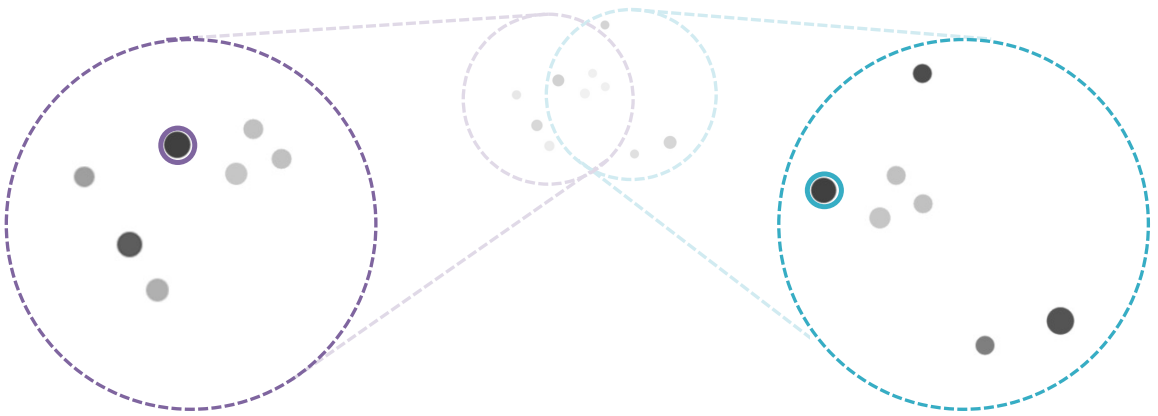
\includegraphics[height=1.5in]{img/oc.png}
\caption{
\label{fig:oc}
An example game board for \texttt{OneCommon}.
}
\end{figure}

\texttt{OneCommon} can be expressed as an MDP $(S,A,T,R)$.
The set of states $S$ for a player is given by their dots $c$ as well as all previous actions
they take in addition to their partner's actions.
The set of actions $A$ are all utterances as well as selections.
The transition model $T: S \times A \to \Delta(S)$ takes the current state and action
and gives us a distribution over the next state,
which includes our partner's response to our action.
Finally, the reward function $R$ gives a reward of -1 for any action other than
select, 10 for selecting the same dot as our partner, and -100 for either
selecting a different dot or not making a selection.

Alternatively, we can express \texttt{OneCommon} as a POMDP $(S,A,T,O,R)$.
We can define the states $S$ to be the probability, if we were to select a dot now,
that our partner would choose the same dot.
Note that this is just one possible definition.
Actions $A$ remain the same as in the MDP formulation.
The transition model $T$ takes the current state and action and returns a distribution over
the next state.
Since we defined the state to be the probability of our partner choosing the same dot,
the transition model is hard to define.
The observation model $O = p(o \mid s, a)$, the probability of observing a partner's
response given the state (just transitioned to) and action.
The reward model $R$ remains the same as in the MDP formulation.

\section{Dynamic Programming Solution}
If all of $|A|,|S|,|O|$ are small, then exact computation of the best policy
is feasible via dynamic programming.
The goal is to maximize the expected utility under your policy,
\begin{equation}
    \argmax_\pi \Es{a_{1:t},s_{1:t}\sim\pi}{\sum_{t=1}^T r(a_t, s_t)}.
\end{equation}
To solve this exactly, we rely on the principle of optimality:
that given a deterministic optimal policy $a^*_{1:T}$ from $\pi^*$ that solves the
above equation, the solution of the ``cost-to-go'' subproblem,
\begin{equation}
    \argmax_{a_{k:T}} \E{\sum_{t=k}^T r(a_t, s_t)},
\end{equation}
is given by $a^*_{k:T}$ from $\pi^*$.
This implies we can solve the original equation for the optimal policy by working backwards
through time, for each state choosing the action that has the best reward / cost:
\begin{equation}
    V(s_t) = \max_{a_t} \sum_{s_{t+1}}r(s_t, a_t) + p(s_{t+1} \mid s_t, a_t)V(s_{t+1})
    = \max_{a_t} Q(s_t, a_t).
\end{equation}
In reinforcement learning, $V$ is the value function and $Q$ the state action value function
(often refered to as just the $Q$ function).
In a fully observed MDP, the time complexity of the dynamic programming solution is $O(T|S|^2|A|)$.
For partially observed POMDPs, exact computation of the optimal policy will often be
intractable, i.e. exponential in actions and observations $O((|A||O|)^T)$,
requiring approximations.

\section{Limited Lookahead Approximation and Rollouts}
In the previous section, we saw how to solve for the optimal policy directly via dynamic programming.
In the case of extremely large state or action spaces,
the dynamic programming solution is intractable even for MDPs.
Rather than computing the exact solution, we can improve tractability via rollouts,
which uses two approximations.
First, instead of working backwards from the end of an episode, we can work backwards
from $k$ steps ahead, referred to as a finite lookahead approximation.
At states $k$ steps ahead, we then use a heuristic model that is cheaper to evaluate
than the value function.
For example, we can use a lookahead of $k=1$ and a value function approximations $\tilde{V}(s_{t+1})$:
\begin{equation}
V(s_t) \approx \max_{a_t} \sum_{s_{t+1}}r(s_t, a_t) + p(s_{t+1} \mid s_t, a_t)\tilde{V}(s_{t+1}),
\end{equation}
while a $k=2$ lookahead approximation would yield 
\begin{equation}
\begin{aligned}
V(s_t)
&= \max_{a_t, a_{t+1}} r(s_t, a_t) + \sum_{s_{t+1}}p(s_{t+1} \mid s_t, a_t)
\left(r(s_{t+1}, a_{t+1}) + \sum_{s_{t+2}}p(s_{t+2} \mid s_{t+1}, a_{t+1})V(s_{t+2})\right)\\
&\approx \max_{a_t, a_{t+1}} r(s_t, a_t) + \sum_{s_{t+1}}p(s_{t+1} \mid s_t, a_t)
\left(r(s_{t+1}, a_{t+1}) + \sum_{s_{t+2}}p(s_{t+2} \mid s_{t+1}, a_{t+1})\tilde{V}(s_{t+2})\right).
\end{aligned}
\end{equation}
There are many choices for the value function approximation $\tilde{V}$,
of which rollouts is a single choice.
In rollouts, we replace the maximization in the dynamic program with an expectation
wrt a suboptimal policy $\pi$ (if we had the optimal policy, approximation would not be necessary):
\begin{equation}
\tilde{V}(s_t)
=\Es{a_t\sim \pi}{\sum_{s_{t+1}}r(s_t, a_t) + p(s_{t+1} \mid s_t, a_t)\tilde{V}(s_{t+1})}
\le \max_{a_t} \sum_{s_{t+1}}r(s_t, a_t) + p(s_{t+1} \mid s_t, a_t)V(s_{t+1})
= V(s_t).
\end{equation}
The second approximation is to approximate the expectation in $\tilde{V}(s_t)$
via Monte Carlo sampling.
We can combine these two approximations by using a $k$-step lookahead and estimating
the value function of future states via rollouts.

The lookahead and rollout approximation trades off bias and accuracy for computational
tractability.
The first lookahead approximation replaces the optimal value function with an approximation,
introducing bias by replacing maxes with expectations.
The second approximation, using rollouts to approximate expectations,
results in variance (a common tradeoff for Monte Carlo methods).

Ignoring the cost of the rollouts themselves, $k$ limited lookahead approaches for MDPs
take $O(k|S|^2|A|)$ computation, while POMDPs take $O((|O||A|)^k)$,
replacing factors of $T$ with $k$.

\section{Monte Carlo Tree Search}
Lookahead methods are a breadth-first method: viewing states and actions as nodes in a tree,
lookahead methods exhaustively explore all states and actions up to depth $k$.
Monte Carlo tree search (MCTS) methods, as well as
partially observable variants such as partially observable Monte Carlo planning (POMCP),
instead take a best-first strategy, expanding the most promising nodes
then approximating their value.

Given a starting tree, MCTS relies on two heuristic policies: a tree and rollout policy.
A simple example of a best-first policy would rely on heuristic estimates of the value function
or $Q$-function for the tree policy,
prioritizing the visitation of states that seem most promising.
Compared to breadth-first, which uniformly assumes that nodes closest to the root are most valuable,
best-first strategies may result in better solutions being found under the same
computational budget (for example with at most $k$ nodes visited).

Similar to limited lookahead methods, best-first relies on heuristic estimates
$\tilde{V}(s)$ of the value function.
Given a starting graph $G$, we must choose a node $n$ on the frontier of $G$, $\delta G$.
The UCT algorithm uses the current value estimate $\tilde(V)(s) + f(s)$,
where $f$ is a function based on visitation statistics that allow practitioners to trade off
exploration and exploitation.
Choosing a node is referred to as the selection phase of tree search.

After selecting the most promising (best) node,
a set of new child nodes are added to the tree in the expansion step.
The simplest expansion step is to add a child of the selected node according to the rollout policy.
The added nodes then have their values estimated via rollouts, called the simulation step.
Finally, value information is backpropagated up the tree.

\section{Symmetry in Tree Search}



\bibliography{bib}

\appendix


\end{document}
